    \section{Complete Backend Class Diagram}
    \label{appendix:uml-class-diagram}

    This appendix provides the complete and detailed UML class diagram for the backend application. It illustrates the static structure of all major classes across the API, Application, and Infrastructure logic layers, showcasing their properties, methods, and relationships.

    Due to its comprehensive nature and to ensure readability, the diagram is presented in two parts. The first part focuses on the core \texttt{Expense} and \texttt{User} management workflows, while the second part details the \texttt{Report} management and real-time notification workflows. Together, they form a single, cohesive model of the system's codebase.

    \subsection{Expense, User, and Storage Management Classes}

    Figure \ref{fig:backclass1-appendix} below details the classes involved in the expense and user management lifecycle. It highlights key components such as the \texttt{ExpenseService}, the \texttt{UserService}, the \texttt{BlobStorageService}, and their corresponding interfaces and implementations. It also shows their direct dependencies on the persistence layer through repositories. 

    The \texttt{ProcessExpenseFromQueue} class contains the implementation executed when the Azure Functions Worker is triggered. Although hosted in an Azure Functions Worker (mentioned in the Physical Architecture Diagram in Figure \ref{fig:physical-architecture-diagram}), its code is logically part of the aPI Layer. 

    Azure Functions act as an adapter for asynchronous system events, just as a Controller acts as an adapter for HTTP requests. The asynchronous flow has already been detailed in Section \ref{sec:physical-architecture}, specifically in the Asynchronous AI Processing Flow section.

    \begin{figure}[H]
        \centering
        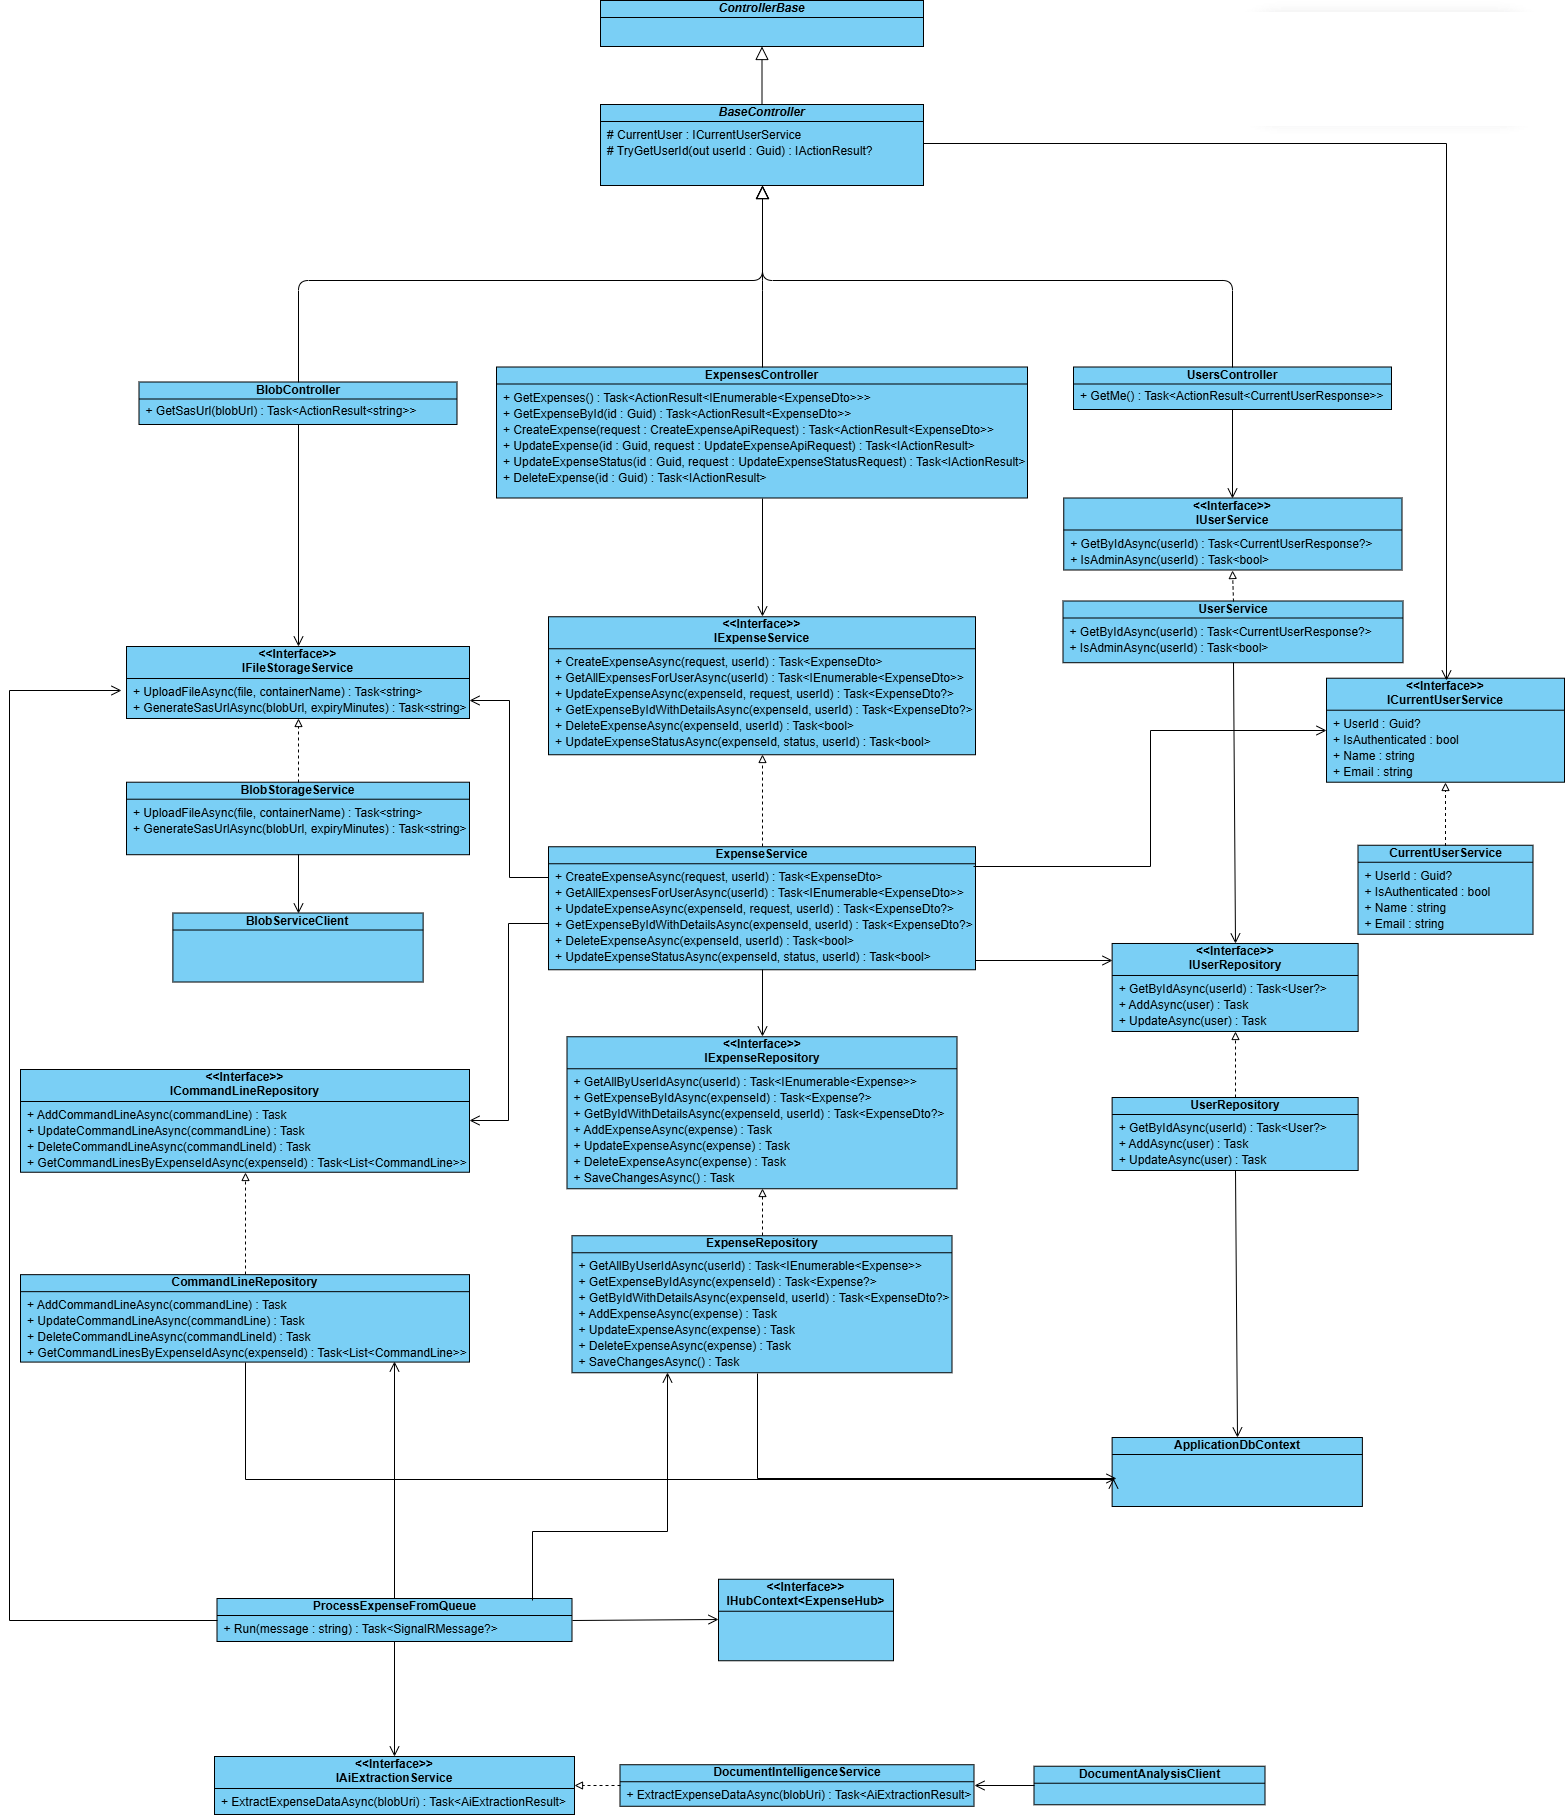
\includegraphics[width=\textwidth]{Images/BackClass/BackClass1.png}
        \caption[UML Class Diagram - Part 1: Expense, User, and Blob Storage Workflows]
        {UML Class Diagram - Part 1: Expense, User, and Blob Storage Workflows. [Own creation]}
        \label{fig:backclass1-appendix}
    \end{figure}

    \newpage

    \subsection{Report Management and Notification Classes}
    
    Figure \ref{fig:backclass2-appendix} below illustrates the classes responsible for the report management lifecycle and real-time communications. It shows the \texttt{ReportsController}, the \texttt{ReportService}, and its dependencies on both \texttt{IReportRepository} and \texttt{IExpenseRepository}, connecting it to the classes shown in Figure \ref{fig:backclass1-appendix}. This diagram also details the components responsible for notifications, including the \texttt{EmailNotificationService} and the \texttt{SignalR ReportHub}.

    \begin{figure}[H]
        \centering
        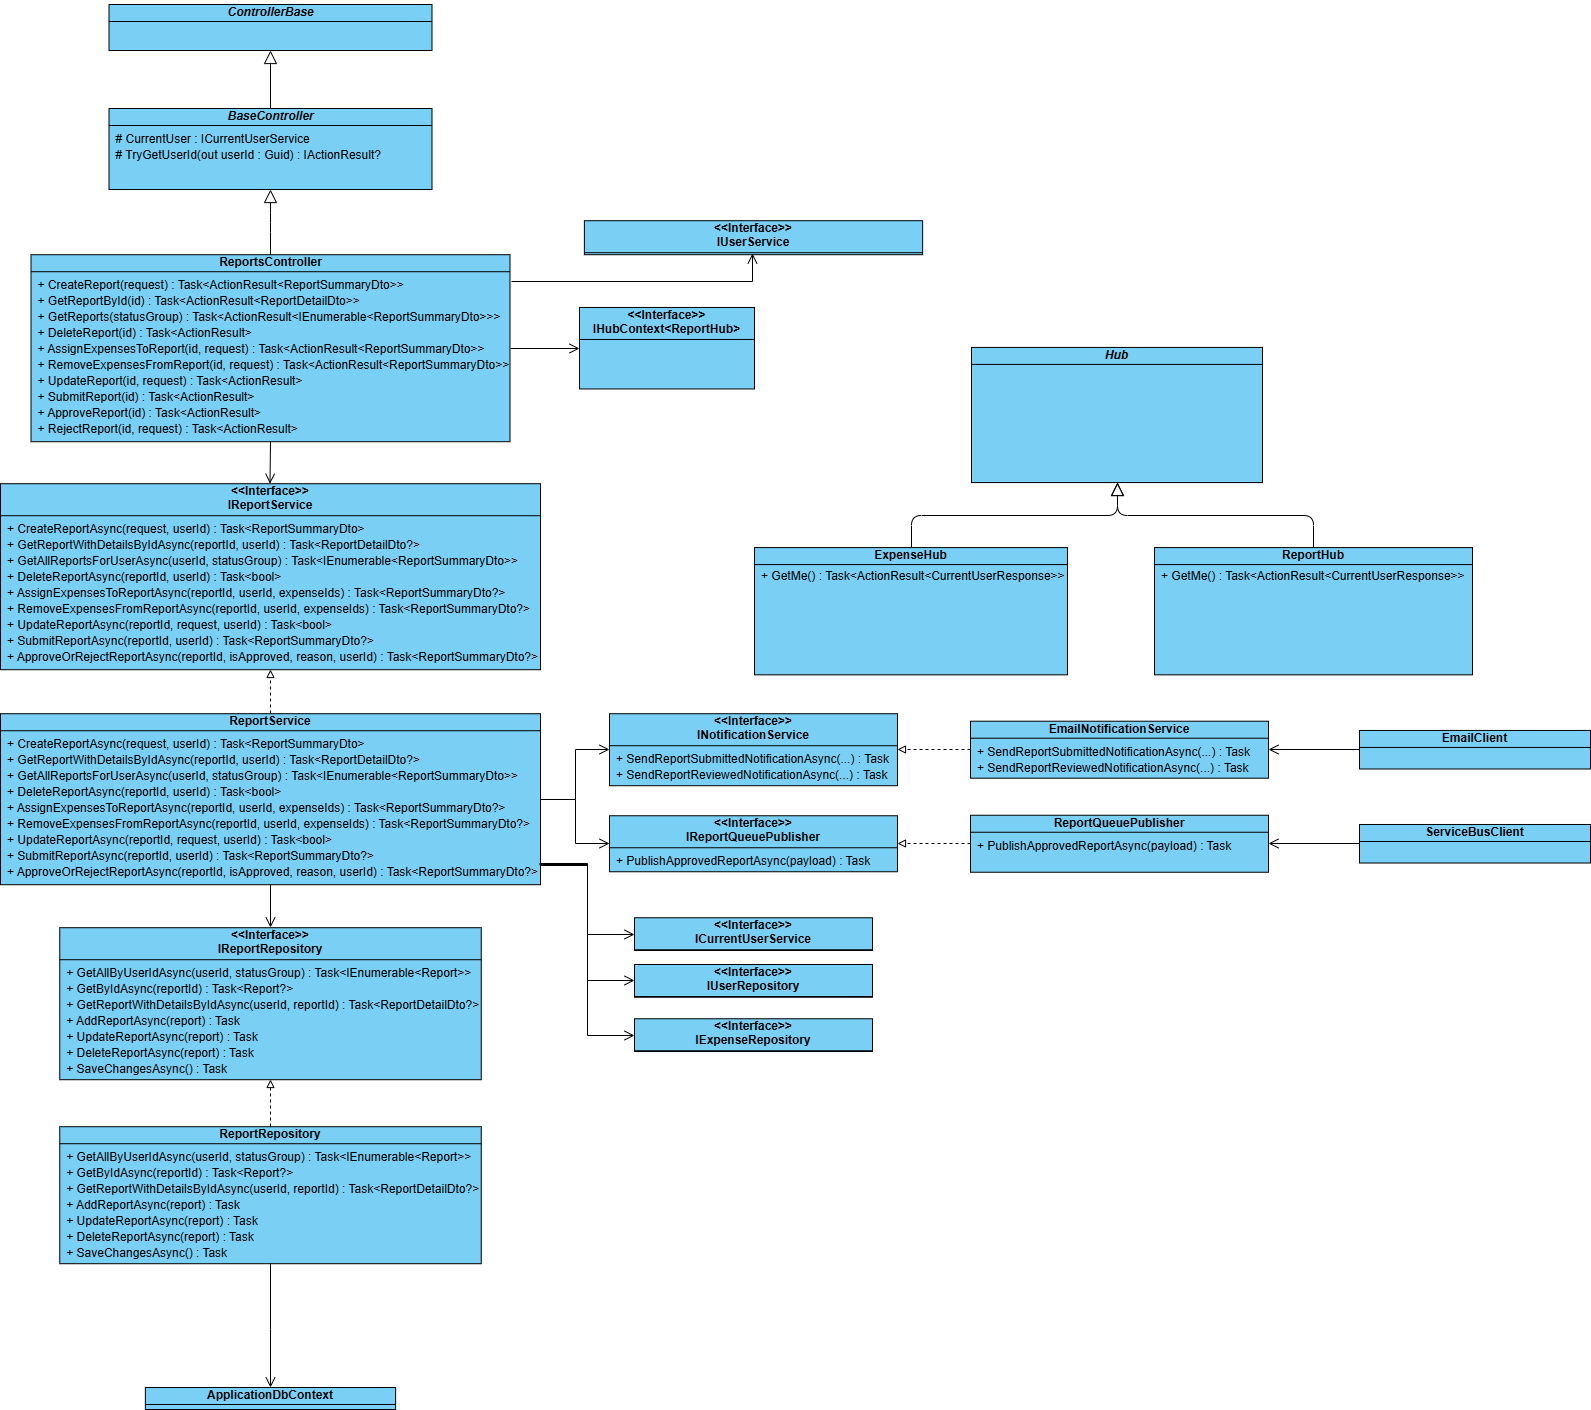
\includegraphics[width=\textwidth]{Images/BackClass/BackClass2.png}
        \caption[UML Class Diagram - Part 2: Report, Notification, and Real-time Hub Workflows]
        {UML Class Diagram - Part 2: Report, Notification, and Real-time Hub Workflows. [Own creation]}
        \label{fig:backclass2-appendix}
    \end{figure} 
